%%%%%%%%%%%%%%%%%%%%%%%%%%%%%%%%%%%%%%%%%%%%%%%%%%%%%%%%%%%%%%%%%%%%%%%%
%                                                                      %
%     File: Thesis_Implementation.tex                                  %
%     Tex Master: Thesis.tex                                           %

%%%%%%%%%%%%%%%%%%%%%%%%%%%%%%%%%%%%%%%%%%%%%%%%%%%%%%%%%%%%%%%%%%%%%%%%

\chapter{Implementation}
\label{chapter:implementation}

\section{Overview}
\label{section:overview}

In this section we describe the implementation details of the Binary Level Serialization, Central Serializer, Receiver, Message Transportation and Deployment and experiences during these implementation.
%%%%%%%%%%%%%%%%%%%%%%%%%%%%%%%%%%%%%%%%%%%%%%%%%%%%%%%%%%%%%%%%%%%%%%%%
\section{Binary Level Serialization}
\label{section:binaryLevelSerialization}

In this section we will present the implementation of the Binary level serialization. In previous chapters it is explained advantages of binary comparing to text-based solutions. we will explain it with experimentations.

Computer languages have their own object types and special serialization algorithms for their object, so when you are working with same language you can easily serialize an object and deserialize it again easily with other application that is written by same language.\\

When we try to work with different computer language and their object types we had problem with serialization.
We can not use standard Java or .Net(C\#) object serialization, because different program languages uses different algoritms for serialization that's why we’ll run into the problem. We can explain that with a simple example. For example Person object in Listing ~\ref{lst:javaperson} binary representation is not the same in .Net(Table \ref{tab:netserilazitaon}) and Java(Table \ref{tab:javaserilazitaon}).

\begin{lstlisting}[caption=Person Object, label=lst:javaperson]
  public class Person
  {
       public String name;
       public int age;
  }
\end{lstlisting}

\begin{table}[]
\centering
\begin{tabular}{lllllllllllllll}
0   & 1   & 0   & 0   & 0   & 255 & 255 & 255 & 255 & 1   & 0   & 0   & 0   & 0   & 0  \\
0   & 0   & 12  & 2   & 0   & 0   & 0   & 73  & 83  & 101 & 114 & 105 & 97  & 108 & 105\\
122 & 97  & 116 & 105 & 111 & 110 & 32  & 116 & 101 & 115 & 116 & 44  & 32  & 86  & 101\\
114 & 115 & 105 & 111 & 110 & 61  & 49  & 46  & 48  & 46  & 48  & 46  & 48  & 44  & 32 \\
67  & 117 & 108 & 116 & 117 & 114 & 101 & 61  & 110 & 101 & 117 & 116 & 114 & 97  & 108\\
44  & 32  & 80  & 117 & 98  & 108 & 105 & 99  & 75  & 101 & 121 & 84  & 111 & 107 & 101\\
110 & 61  & 110 & 117 & 108 & 108 & 5   & 1   & 0   & 0   & 0   & 25  & 83  & 101 & 114\\
105 & 97  & 108 & 105 & 122 & 97  & 116 & 105 & 111 & 110 & 95  & 116 & 101 & 115 & 116\\
46  & 80  & 101 & 114 & 115 & 111 & 110 & 2   & 0   & 0   & 0   & 21  & 60  & 110 & 97 \\
109 & 101 & 62  & 107 & 95  & 95  & 66  & 97  & 99  & 107 & 105 & 110 & 103 & 70  & 105\\
101 & 108 & 100 & 20  & 60  & 97  & 103 & 101 & 62  & 107 & 95  & 95  & 66  & 97  & 99 \\
107 & 105 & 110 & 103 & 70  & 105 & 101 & 108 & 100 & 1   & 0   & 8   & 2   & 0   & 0  \\
0   & 6   & 3   & 0   & 0   & 0   & 4   & 74  & 111 & 104 & 110 & 32  & 0   & 0   & 0  \\
11  &     &     &     &     &     &     &     &     &     &     &     &     &     &    \\
\end{tabular}
\caption[.Net Serialization Person Object]{.Net Serialization Person Object}
\label{tab:netserilazitaon}
\end{table}

\begin{table}[]
\centering
\begin{tabular}{lllllllllllllll}
  -84 & -19 & 0   & 5  & 115 & 114 & 0   & 23   & 106 & 97  & 118 & 97  & 97  & 112  & 112 \\
  108 & 105 & 99  & 97 & 116 & 105 & 111 & 110  & 55  & 46  & 80  & 101 & 114 & 115  & 111 \\
  110 & 79  & -70 & 94 & 85  & -31 & -32 & -110 & 90  & 2   & 0   & 2   & 73  & 0    & 3 \\
  97  & 103 & 101 & 76 & 0   & 4   & 110 & 97   & 109 & 101 & 116 & 0   & 18  & 76   & 106 \\
  97  & 118 & 97  & 47 & 108 & 97  & 110 & 103  & 47  & 83  & 116 & 114 & 105 & 110  & 103 \\
  59  & 120 & 112 & 0  & 0   & 0   & 32  & 116  & 0   & 4   & 74  & 111 & 104 & 110  &     \\
\end{tabular}
\caption[Java Serialization Person Object]{Java Serialization Person Object}
\label{tab:javaserilazitaon}
\end{table}

After that experiment we decided to use our algoritm instead of using stardard serializer for Java or .Net that both languages could understand and easily serialize or deserialize.\\

The binary format is always the result of serializing data in each language, with a tag, the number of bytes that follow and the serialized content. Recovering the serialized data is simply testing the tag to find the data type and then using the number of bytes and the serialized content.\\

A message to be sent should be an object (in Java or .Net) that should provide a serialization method, which basically builds a serialized message (an array of bytes) by sucessively adding each of its components, serialized. This is done by invoking the methods of the serialization class for primitive data or by recursively invoking the serialization method of structured objects that constitute the message.\\

Instead of every class has their own serializer class, we implemedted idea of centralizing the “object of primitive type to a sequence of bytes” and vice-versa methods in a single class is to avoid the need for every class to have these methods. Since they are static (they receive an object and return bytes, or vice versa), they can simply be concentrated in a static class (no instances) and invoked from anywhere.\\

The methods to serialize can receive a primitive object (integer, Boolean, etc) and an array of bytes, returning the array of bytes with the serialized object’s bytes appended. Therefore, each serialization method grows the byte array. When the user wants to send a message, that message needs to be an instance of a class that has a method that knows how to serialize it, by invoking the serialization methods of the static class for each of its variables. This needs to be programmed by the use and is similar to the programming language’s serialization methods.\\

We will show some examples of primitive type serialization.

\begin{figure}[!htb]
  \centering
  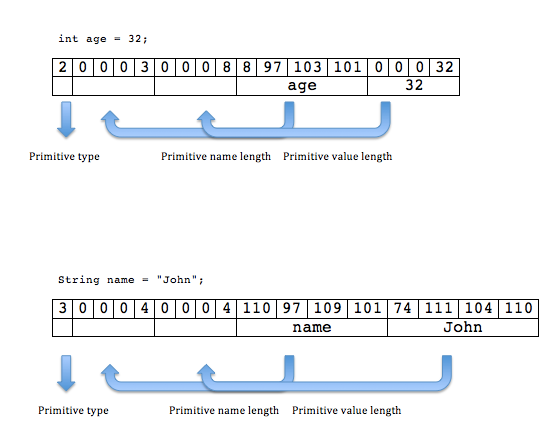
\includegraphics[width=0.9\textwidth]{Figures/binary.png}
  \caption[Examples of primitive type serialization.]{Examples of primitive type serialization.}
  \label{fig:examplebinary}
\end{figure}

To examine the performance in serializing structed data in binary and text-based data(XML,JSON), an experiment was designed using following hardware and software:
\begin{itemize}
\item 	Hardware: IMac(by Apple Inc.) with Intel Core i7 1,7 GHz and 8GB memory.
\item 	Operation System: Mac OS X version 10.11.4.
\item 	Java: version 1.8.
\end{itemize}

Current version of object serialization libraries were selected shown in the following:
\begin{itemize}
\item 	JAXB Serializer for XML serialization.
\item   Jackson Serializer for JSON serialization.
\item 	OpenEXI for XML compression
\end{itemize}
The experiment was  designed as follows:
\begin{itemize}
\item 	Ten kinds of query were prepared for weathercast provider. They were queries with ten size of weather: 0, 100, 200, 300, 400, 500, 600, 700, 800, 900 city weathercast query
\item   The serialized file was measured and the execution time was measured using System.currentTimeMillis() shown in Listing ~\ref{lst:timeserialize}.
\end{itemize}

\begin{lstlisting}[caption=Serialization program for testing, label=lst:timeserialize]
          long start = System.currentTimeMillis();
          Query q = new Query();
          for (int i = 0; i < 900; i++) {
              q.weathers.add(new Weather());
          }
          json = serialize(query);
          long end = System.currentTimeMillis();
          double time  =  (double) (end-start);
\end{lstlisting}

The avarage size of ten kinds of serialized files given in Table ~\ref{tab:binaryyy}.
\begin{table}
\centering
\begin{tabular}{ p{5.50cm} p{5.50cm} }
\toprule
\multicolumn{1}{l}{\textbf{Format}} & \textbf{Avarage (bytes)}\\
\midrule
\textbf{XML}    & 62008\\
\textbf{EXI}    & 3030\\
\textbf{JSON}   & 32036\\
\textbf{Binary} & 35984\\

\bottomrule
\end{tabular}
\caption[Sizes (in bytes) of several resource representations.]{Sizes (in bytes) of several resource representations.}
\label{tab:binaryyy}
\end{table}

From the point of the avarage size, the largest is a serialized file using XML.

From quantative aspects, the size of binary-based serialized data is better than XML-based and JSON-based serialiation since there is no schema required.


%%%%%%%%%%%%%%%%%%%%%%%%%%%%%%%%%%%%%%%%%%%%%%%%%%%%%%%%%%%%%%%%%%%%%%%%

\section{Receiver and Compliance}
\label{section:compliance}

Compliance is done at the binary level, with primitive components. It is done both  Receiver's operations formal argument and received message. Only the components that match are assigned to the formal argument of the operation. Two partners will be able to communicate as long as the sender complies with receiver and the receiver conforms to what the sender expects and it supports all the features that the sender requires.\\

When a suitable operation is found, another array of bytes is built from both the message and the formal argument then receiver matches components in the formal argument, if it matches it uses the message ones but if not matched by any in the message, use the ones already in the formal argument. The system  also support optional components which use the formal argument component if none in the message matches it. Therefore, the serialization methods in the static serialization class should include the name of the component, whether it is mandatory, the type(encoded in the tag) and the value. Each primitive data type can have mandatory annotation. Messages sent use only with mandatory values. Serialized formal arguments can use both mandatory and non-mandatory.The receiver has always a default value for the message, so for the data that don't mandatory annotation it will always use default value.\\  

To clarify the compliance, the idea is to serialize the argument (only one, but it can be structured) of each operation of a service(receiving object). This acts like a default value, against which the message received is matched. A service receiving a message matches it against the argument of each operation, until it finds one, assigns the message to that argument (partial assignment) and runs the operation, returning eventually a result.\\

When checking for compliance, a component in the message with the same name as a component in the operation’s argument matches it and can be assigned to it (if the message complies with the argument, as a whole). If not, it is ignored. If a component in the argument is not matched by any of the message’s components and is optional , retains the argument’s value (which acts as a default value). If all non-optional  components in the argument are matched, there is compliance, the matching components of the message are assigned to those of the argument with the same name and those that do not match are ignored. Thus the designation partial assignment.\\

We have given an example for mobile phone and weathercast provider interaction in previous sections. Now lets demonstrate how it will work in our solution. Again your mobile phone creates a query and then sends it to weathercast provider. After a message arrived to weathercast provider. it calculate the response message and sent it to your mobile phone and it displays you the result. Here again your phone application is developed with JAVA and weathercast provider is developed with.Net technology. In our solution your mobile will create a binary message and send it to weathercast provider using websocket or HTTP2 technology. in Listing x shows very simple example message that can be sent to weathercast provider. So it is a weather object which will be transformed to binary and transferred to weathercast provider. In weathercast provider has Receiver class and it has different methods with @AvaliableMethod notation and they are responsible to be matched when compliance is happening. After a message arrives from your mobile phone, The system checks your message and methods in Receiver class and if one is matched it invokes its method and return response code. Let's say we have Weather1 class in Receiver and it has primitive values as in Listing xx. As it seen all primitive data has Mondatory notation so in that case type of primitive, name of primitive and value of primitive must be the same to be matched. if we have city name Braga instead of Lisbon it will not matched and the result will not be returned. Lets say we have another Weather2 class as in Listing and in that class not all primitive values have mandatory annotation. So now when your phone send message. it is only important city information which is mondatory. Lets say we are sending weather object as in Listing cc, and receiver has Weather2      

%%%%%%%%%%%%%%%%%%%%%%%%%%%%%%%%%%%%%%%%%%%%%%%%%%%%%%%%%%%%%%%%%%%%%%%%
\section{Message Transportation}
\label{section:messageTransfer}

Transferring the array of bytes from sender to receiver requires a binary channel like Web Sockets(HTTP2) or
more classical way by encoding and decoding the binary array with BASE64 and then use typical HTTP-based
solutions (Web Services or REST). The classical solution is of course non-optimal compared to the other ones,
but it can easier to implement given existent tools.\\

Message Transportation in this solution is done with essentially JavaScript and WebSockets [14], to circumvent some of the limitations of HTTP.
The most important issue is that finally humans are also becoming direct Web producers and not merely clients of servers.\\

Web Sockets [44] are fundamental in the efficient support for binary data removes this restriction, increases performance.
They use the protocol upgrade feature of HTTP and
provide a substantial degree of compatibility with existing systems. Part of the HTML5 world, servers and firewalls are
increasingly supporting them and removes this restriction, adds binary support and increases performance.

\begin{figure}[!htb]
  \centering
  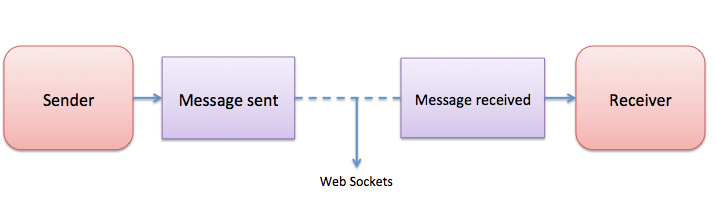
\includegraphics[width=0.5\textwidth]{Figures/websocket.png}
  \caption[Message Transportation.]{Message Transportation.}
  \label{fig:websocket}
\end{figure}

%%%%%%%%%%%%%%%%%%%%%%%%%%%%%%%%%%%%%%%%%%%%%%%%%%%%%%%%%%%%%%%%%%%%%%%%

\section{Deployment}
\label{section:deployment}

The solution is developed and in two different language. They are .NET and Java and deployed Microsoft Azure Cloud. That's way we can
have 2 different provider and .Net client can send message to Java provider over the cloud by using WebSockets and also Java client can
send message to .Net provider. Using Microsoft Azure Cloud allowed us to test project in cloud enviroment
